\chapter{Git on it}

\begin{fullwidth}

{\em\small For our purposes in MSAN, we're going to ignore most of the nontrivial capabilities that programmers use routinely, such as branching and merging. Git is extremely  complicated and would not be my first choice if it weren't for the excellent {\tt github.com}.}

\section{Introduction to revision control}


{\em Revision control} is a mechanism to track all changes to a set of files, which we typically associate with the project. The file status call a {\em repository} and at any given time, my computer has lots and lots of these repositories. 

A {\tt git} repository instance is just a directory on your disk that also happens to have a {\tt .git} (hidden) directory, which is effectively a complete database of everything that's happened to the repository since it was created with {\tt git init} (or you {\tt clone}'d it from somewhere). Every time you {\em commit} a change (file edit, file add, file delete, ...) to the repository, the revision control system tracks a patch called the {\em diff} that indicates essentially how to edit the first file version in order to arrive at the current file version. Storing just the differences is very space efficient and  lets the revision control system apply the same set of changes to a file on a different computer to keep them both in sync.  

Having a complete list of changes is extremely useful. For example, here is a chunk taken out of the middle of my commits on the ANTLR repository as shown by SourceTree:

\scalebox{.85}{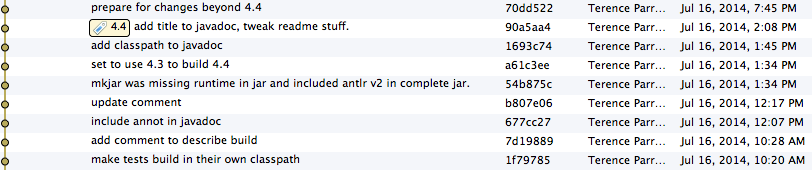
\includegraphics{figures/commits.png}} 

If you want to throw out the repository, just remove the entire subtree from your disk. There is no central server to notify. Every repository instance is a complete copy so you could have, for example, 10 versions of the repository cloned from an original sitting on the same disk.

After you create a repository, you can add all sorts of files but git ignores them until you add them. When you add files or modify files already known to git, they are in the so-called staging area (this used to be called the index). You can have whatever other files you want laying around, such as development environment preference files. Git will simply ignore them unless you add them. This is different than other revision control systems that insist upon knowing about and managing everything under a particular subtree. I like that feature.

\subsection{Does a solo programmer need revision control?}

If you are working solo, from a single machine, and you have a regular backup mechanism in your development environment or from the operating system like Time Machine (OS X), you can get away without a formal revision system.

There are lots of important operations that can be faked without a revision system. It's a good idea to keep track of versions of the software that work or other milestones. In the old days, people would make a copy of their project directory corresponding to important milestones like "Added feature X and it seems to work." You can do comparisons using a diff tool in between directories.

Whether your IDE does it or a revision control system does it, I find it very important to look back at recent changes to see what changes have introduced a bug. Or I decide to abandon a small piece of what's going on and flip a file back to an old version.

A good example of use of a repository is the repository for this course:

\href{https://github.com/parrt/msan501}{\textcolor{blue}{https://github.com/parrt/msan501}}

\noindent It contains all the changes that I've made since I started teaching this course.

These days, revision control systems are meant to be used among multiple computers and multiple developers, but they are still useful even on a single machine.

\subsection{Solo programmer, sharing across machines}

In order to work on that software from your home machine and a laptop for example, you have to make copies. That introduces the possibility that you will overwrite the good version of your software. Or, you will forget that you had made changes on your laptop but have now made a bunch of changes on your desktop. Resolving things can be tricky and error-prone.

As a side benefit, pushing your repository to a remote server gives you a backup automatically.

\subsection{Multiple programmers}

When you add another person to the project, people end up mailing code around but it's difficult to perform a merge. My experience watching students do this reveals that two versions of the software always appear. Both students shout that their version is better and that the other version should be abandoned.

In my experience, no matter how you try to fake multiple states of the source code and share, merging changes to work on the same code base is a nightmare.

Once in a while I go back and I look at the history of changes. Sometimes I want to know who screwed this up or I want to see the sequence of changes that I made or that were made by somebody else.

Every single commercial developer I know uses revision control at work. Every company you will encounter uses it. For that reason alone, you need to learn revision control to be functional in a commercial setting.

\section{Cloning an existing repository}

Fire up SourceTree and use the file menu {\tt New / Clone} option. You will see:
\vspace{5mm}

\begin{table}[htp]
\begin{center}
\begin{tabular}{cc}
Clone repo using SourceTree & Using URL {\tt git@github.com:...} from web \\
\scalebox{.5}{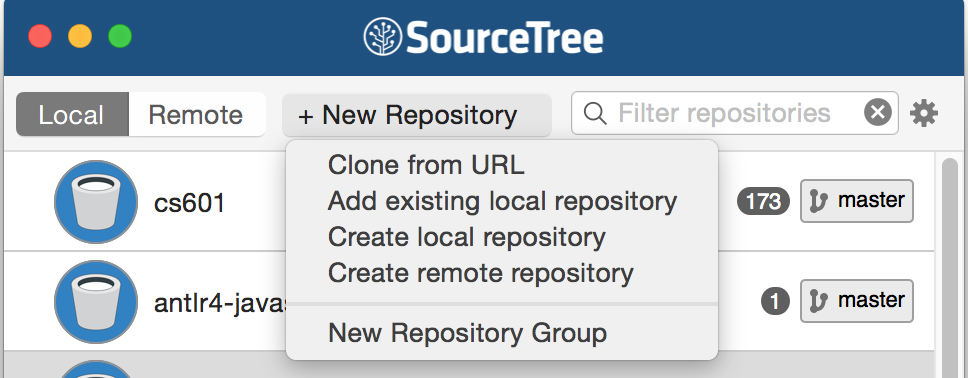
\includegraphics{figures/srctree-clone.png}} & \scalebox{.2}{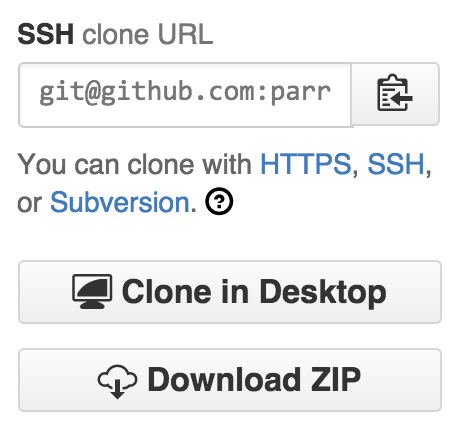
\includegraphics{figures/srctree-url.png}} \\
\end{tabular}
\end{center}
\end{table}%
\vspace{5mm}

You can clone that starter kit into any directory you like, but you should probably name it {\tt msan501} or something similar like {\tt parrt-rocks}.
\vspace{5mm}

\scalebox{.5}{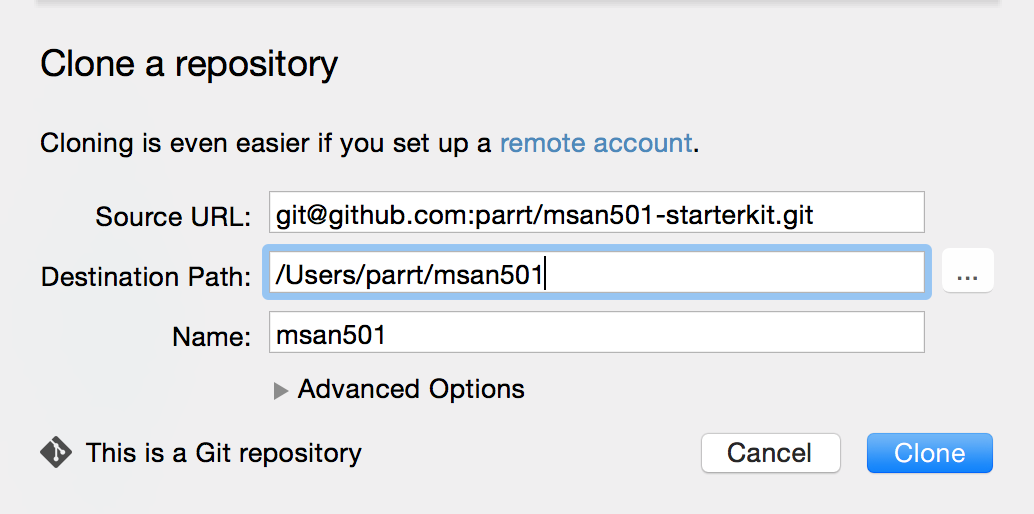
\includegraphics{figures/srctree-url2.png}}
\vspace{5mm}

You'll then see the status of the repository; click on the {\tt master} branch in the left gutter:
\vspace{5mm}

\scalebox{.8}{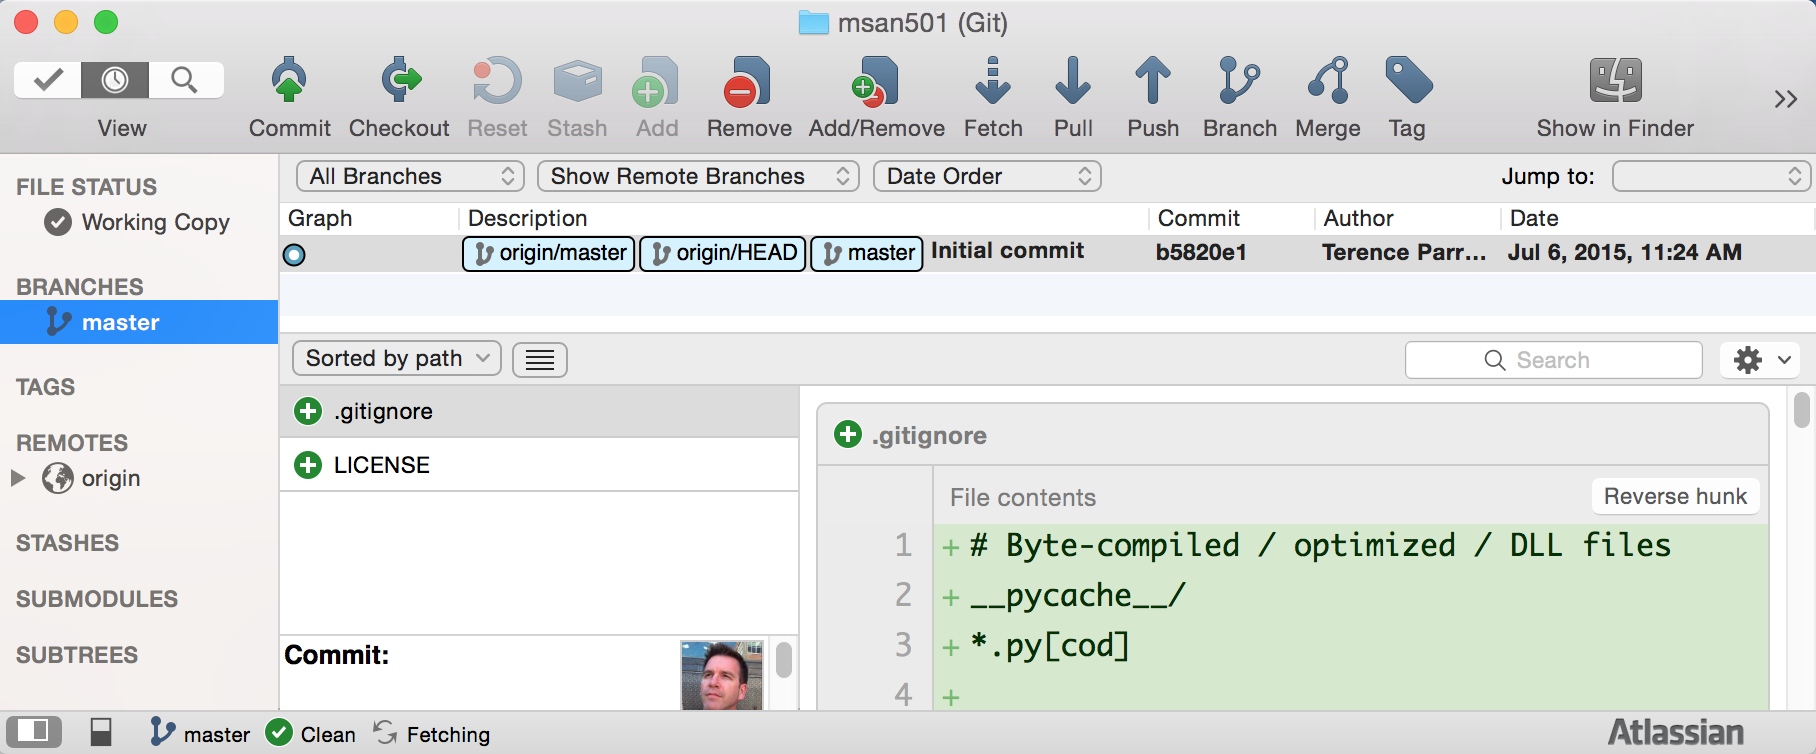
\includegraphics{figures/srctree-repo.png}}

\end{fullwidth}
